\documentclass[convert={outfile=\jobname.png}]{standalone}
\usepackage{base}
\usepackage{draw}
\usepackage{code}

\begin{document}

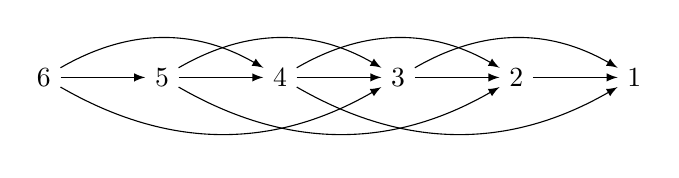
\begin{tikzpicture}
\node (1) at (-1.5*1,0) {1};
\node (2) at (-1.5*2,0) {2};
\node (3) at (-1.5*3,0) {3};
\node (4) at (-1.5*4,0) {4};
\node (5) at (-1.5*5,0) {5};
\node (6) at (-1.5*6,0) {6};
\draw[->, >=latex] (2) to[] (1);
\draw[->, >=latex] (3) to[] (2);
\draw[->, >=latex] (4) to[] (3);
\draw[->, >=latex] (5) to[] (4);
\draw[->, >=latex] (6) to[] (5);
\draw[->, >=latex] (3) to[bend left] (1);
\draw[->, >=latex] (4) to[bend left] (2);
\draw[->, >=latex] (5) to[bend left] (3);
\draw[->, >=latex] (6) to[bend left] (4);
\draw[->, >=latex] (4) to[bend right] (1);
\draw[->, >=latex] (5) to[bend right] (2);
\draw[->, >=latex] (6) to[bend right] (3);
\end{tikzpicture}

\end{document}